\documentclass{article}

\usepackage[a4paper, margin=1in]{geometry}
\usepackage[onehalfspacing]{setspace} % Correct 1.5 line spacing

\usepackage{graphicx}  % Figures
\graphicspath{{../figures/}}

\usepackage{fontspec}  % Fonts
\usepackage{helvet}
\usepackage{newpxtext,newpxmath}
\defaultfontfeatures{Scale=MatchLowercase, Ligatures=TeX}

\usepackage{url}
\usepackage[pdfusetitle]{hyperref}
\usepackage{titlesec}      % Modify title/section/chapter commands
\usepackage{mathtools}     % Various maths related commands
\usepackage{gensymb}       % \degree symbol
\usepackage[thinc]{esdiff} % Derivatives
\usepackage{booktabs}      % \toprule, etc., in tables

% SI units
\usepackage{siunitx}   
\sisetup{separate-uncertainty=true,number-mode=text,detect-weight=true}
\DeclareSIUnit\belm{Bm}
\DeclareSIUnit\belw{BW}
\DeclareSIUnit\beli{Bi}
\DeclareSIUnit\belz{BZ}

% https://tex.stackexchange.com/a/43009
\DeclarePairedDelimiter\abs{\lvert}{\rvert}%
\DeclarePairedDelimiter\norm{\lVert}{\rVert}%

% Caption figures
\usepackage{caption}
\DeclareCaptionFont{captionlabelfont}{\bfseries \sffamily}
\DeclareCaptionFont{captiontextfont}{\sffamily}
\captionsetup{labelfont=captionlabelfont, textfont=captiontextfont}

% Change footnote style
\renewcommand{\thefootnote}{\fnsymbol{footnote}}

% Fancy header/footer
\usepackage{fancyhdr}
\pagestyle{fancy}
\renewcommand{\sectionmark}[1]{\markright{\thesection . #1}}
\fancyhf{}
\lhead{\fancyplain{}{\thepage}}
\rhead{\fancyplain{}{\textit{\rightmark}}}

% Bibliography
\usepackage[backend=biber, style=phys, natbib=true,
			url=false, isbn=false, doi=false, eprint=false,
			autocite=superscript, urldate=long, maxcitenames=2]{biblatex}

\addbibresource{references.bib}

\newcommand\mytitle    {Millimetre-Wave Cloud Profiling Radar}
\newcommand\mysubtitle {Pre-Project Review}
\newcommand\myauthor   {180014855}
\newcommand\mydate     {\today}
\newcommand\mymodule   {PH4111}
\newcommand\mywordcount{1702}

\title {\mytitle}
\author{\myauthor}
\date  {\mydate}

\begin{document}

\begin{titlepage}
	\centering
	{
\includegraphics[width=0.3\textwidth]{uos-logo}}
	\par
	{\LARGE\bfseries University of St. Andrews\par}
	{\LARGE School of Physics and Astronomy\par}
	\vspace{1.5cm}
	{\huge\bfseries\mytitle\par}
	{\Large\mysubtitle\par}
	\vspace{2cm}
	{\Large\myauthor\par}
	{\large\textbf{Module:} \mymodule\par}
	{\large\textbf{Word count:} \mywordcount\par}
	\vfill
	{\large\today\par}
\end{titlepage}

\section{Introduction}
Meteorological radar systems provide great insight into weather phenomena, allowing for improved forecasts and for meteorologists to study clouds on a large scale. Clouds have a great influence on Earth's surface temperature, being able to both reflect and trap solar radiation, thus it is essential to study clouds to predict climate change. However, the high cost of conventional pulse Doppler radars limits deployment and hence the amount of cloud profiling data that can be gathered. One of the most significant factors is due to the high peak power requirement since, for the most of the time, the radar is not transmitting.
Much attention has been devoted to frequency-modulated continuous wave (FMCW) radars, which, as they continuously transmit, do not require as much peak power and hence cheaper amplifiers can be used.

Cloud particles are typically much smaller than millimetre waves, thus the Rayleigh backscattering approximation may be applied to greatly simplify calculations. The other key advantage is the high radar cross-section (RCS), a quantity indicating how much energy is reflected by a target. Figure \ref{fig:RayleighCurve} illustrates that, as one increases particle size and incident frequency, the RCS increases. However, at wavelengths comparable to particle size, this relationship is nonlinear and better described by Mie scattering.

In addition, millimetre waves are strongly attenuated by molecules in the atmosphere, limiting their maximum useful range to a few tens of kilometres. Frequencies around \SI{35}{\giga\hertz} and \SI{94}{\giga\hertz} are often used in cloud radars, since the atmospheric attenuation is at a local minimum allowing the entire range of the cloud to be probed (Fig. \ref{fig:Attenuation}).

\begin{figure}
	\centering
	\begin{minipage}{0.48\textwidth}
		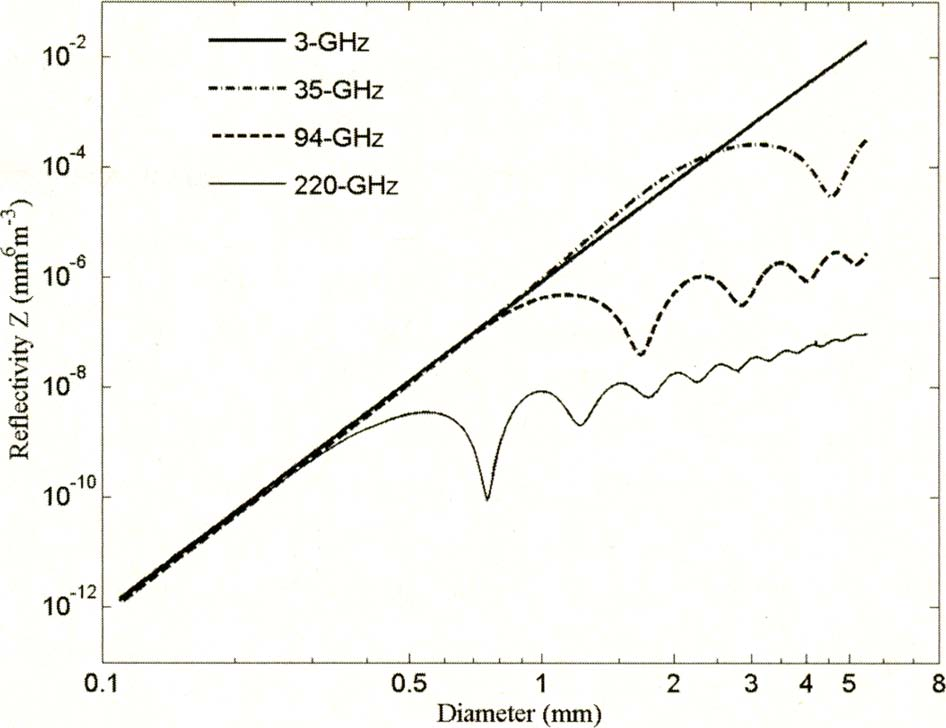
\includegraphics[width=0.98\textwidth]{rayleigh-2}
		\caption{Reflectivity of spherical particles as a function of diameter for various frequencies.\supercite{KolliasFrontier} The Rayleigh backscattering approximation is only applicable in the linear regime, where the particle size is small relative to the wavelength. As the ratio between particle size and wavelength increases, the behaviour is more accurately described by Mie theory.\supercite{POMRRayleighScattering}}
		\label{fig:RayleighCurve}
	\end{minipage}
	\hfill
	\begin{minipage}{0.48\textwidth}
		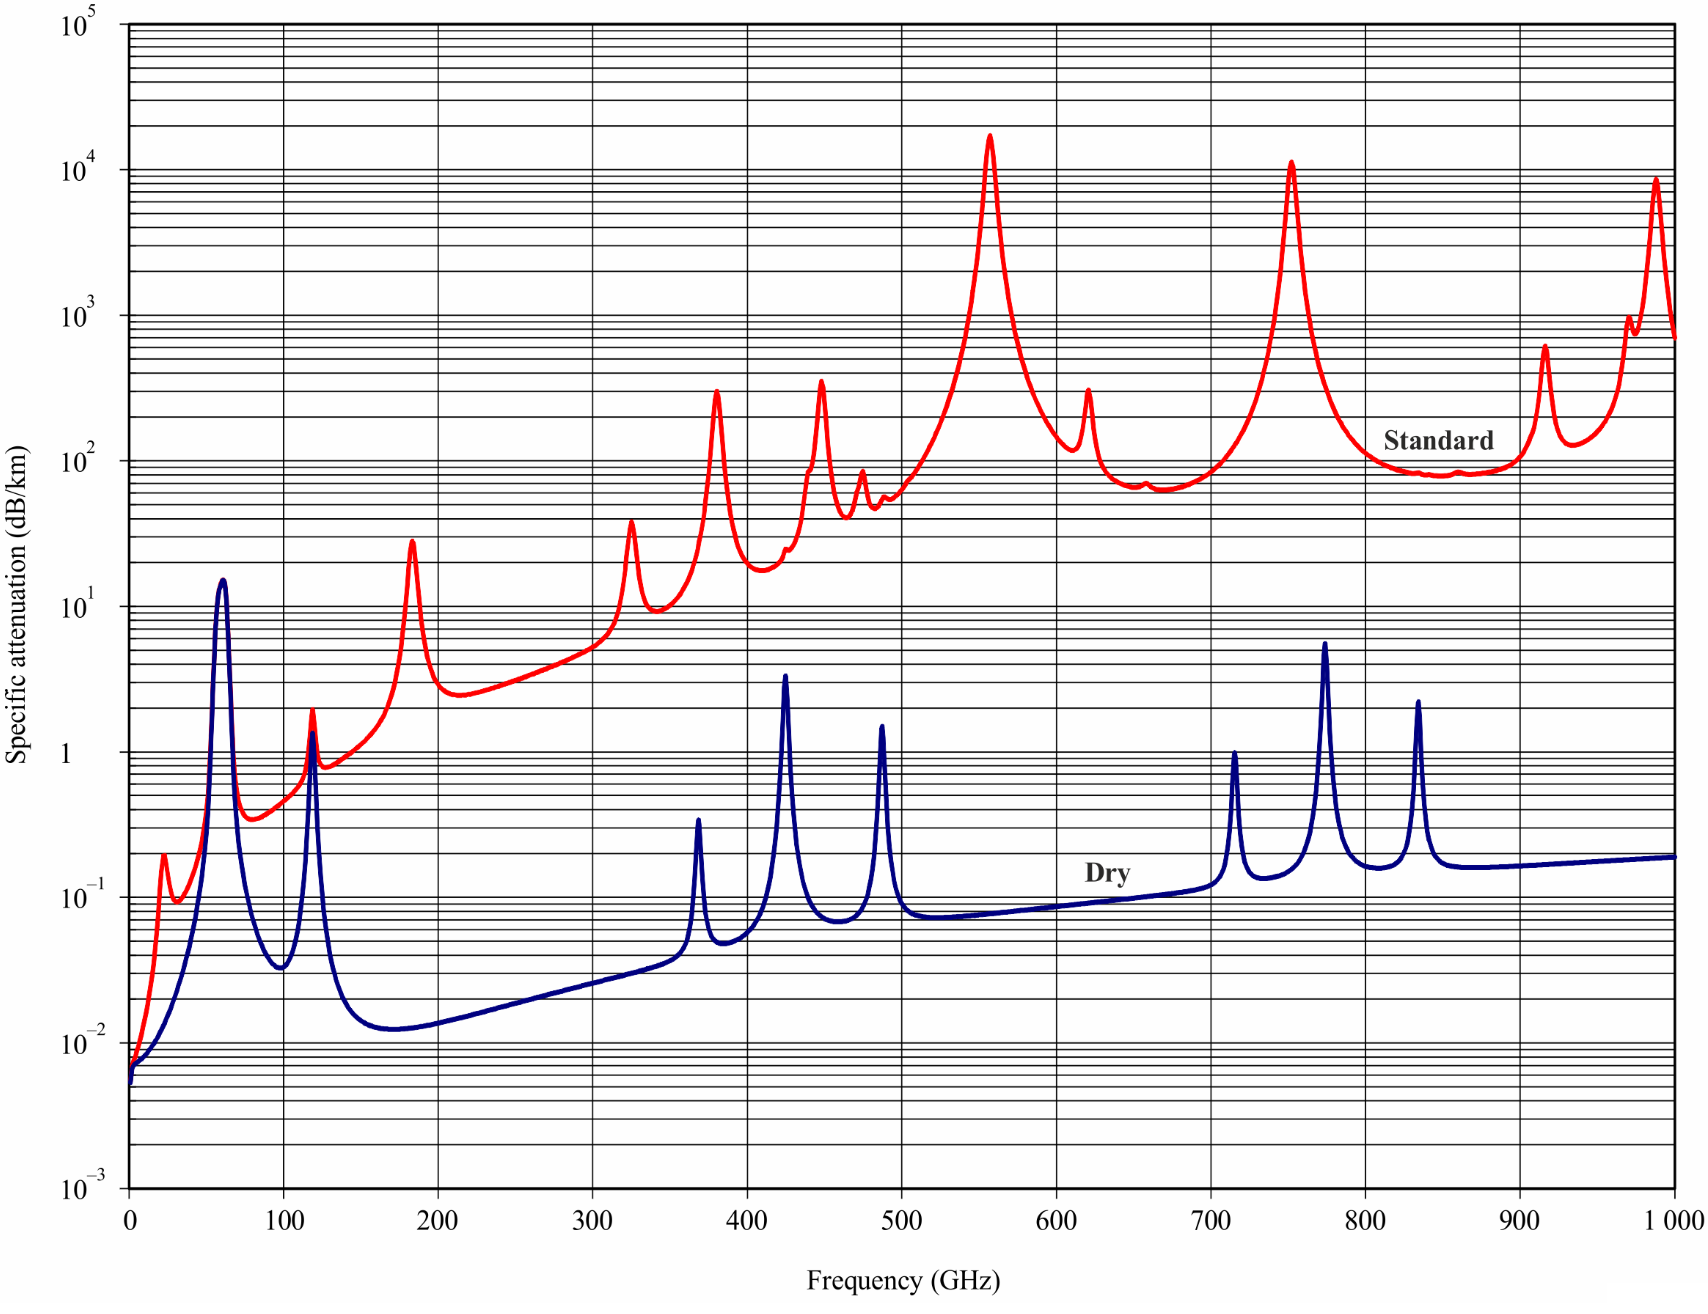
\includegraphics[width=0.98\textwidth]{attenuation}
		\caption{Atmospheric attenuation as a function of radar frequency for dry and standard atmosphere conditions.\supercite{ITURAttenuation} Peaks corresponding to absorption by molecules in the atmosphere are visible throughout.}
		\label{fig:Attenuation}
	\end{minipage}
\end{figure}

\section{Meteorological radar}

\subsection{Radar range equation}
The most important equation in radar is the \textit{range equation}, which, in its simplest form, links the power received to the power transmitted by a prefactor containing target range, wavelength, RCS, and gain. For a point target, the range equation takes the form
\begin{equation}
	P_r = \frac{P_t G_t G_r \lambda^2}{(4 \pi)^3 r^4} \sigma, \label{eqn:PointTarget}
\end{equation}
where \(\sigma\) is the RCS, \(P_t\) and \(P_r\) are the transmitted and received power, \(G_t\) and \(G_r\) are the transmit and receive antenna gains, \(\lambda\) is the radar wavelength, and \(r\) is the distance to the target.

For distributed targets such as rainfall or particles in a cloud, the radar cross-section becomes \(\sigma = V\eta\), where \(V\) is the volume sampled by the radar and \(\eta\) is the volume reflectivity.
One can show that\supercite{RadarHandbookMeteo}
\begin{equation}
	V = \frac{1}{8} \pi r^2 \theta \phi c \tau,
\end{equation}
where \(\theta\) and \(\phi\) are the angular beamwidths, measured from the centre to the \(-\)\SI{3}{\decibel} point of the main lobe. \(\tau\), in the case of FMCW radar, is the reciprocal of the chirp bandwidth (?explain?).
The volume reflectivity is essentially the sum of the radar cross-sections per unit volume for each target in the volume. Under the Rayleigh backscattering approximation, it takes the form\supercite{RadarMeteorology}
\begin{equation}
	\eta = \sum_i{\sigma_i} = \frac{\pi^5}{\lambda^4} \abs{K}^2 \sum_i{D_i^6} = \frac{\pi^5}{\lambda^4} \abs{K}^2 Z,
\end{equation}
where \(Z\) is the radar reflectivity factor and \(\abs{K}^2\) is a constant dependent on phase (water, ice), temperature, and frequency. \(Z\) is by far the most important term since, when combined with range data, it allows one to distinguish cloud types or determine the precipitation intensity.

Combining the expressions for \(V\) and \(\eta\) yields the radar range equation for meteorological targets,\supercite{RadarHandbookMeteo}
\begin{equation}
	P_r = \frac{P_t G_t G_r \lambda^2}{(4 \pi)^3 r^4} \cdot \frac{1}{2\ln{2}} \cdot \frac{\pi r^2 \theta \phi c \tau}{8} \cdot \eta = \frac{P_t G_t G_r \lambda^2 \theta \phi c \tau}{1024 (\ln{2}) \pi^2 r^2} \eta = \frac{P_t G_t G_r \theta \phi c \tau \pi^3 \abs{K}^2}{1024 (\ln{2}) \lambda^2 r^2} Z,
	\label{eqn:MeteoRange}
\end{equation}
where we have added a factor \(1/(2\ln{2})\) as suggested by Probert-Jones (1962)\supercite{ProbertJones} to account for the fact that antenna gain is not uniformly distributed across the sample volume.

\subsection{Frequency-modulated continuous wave radar}
\begin{figure}
	\centering
	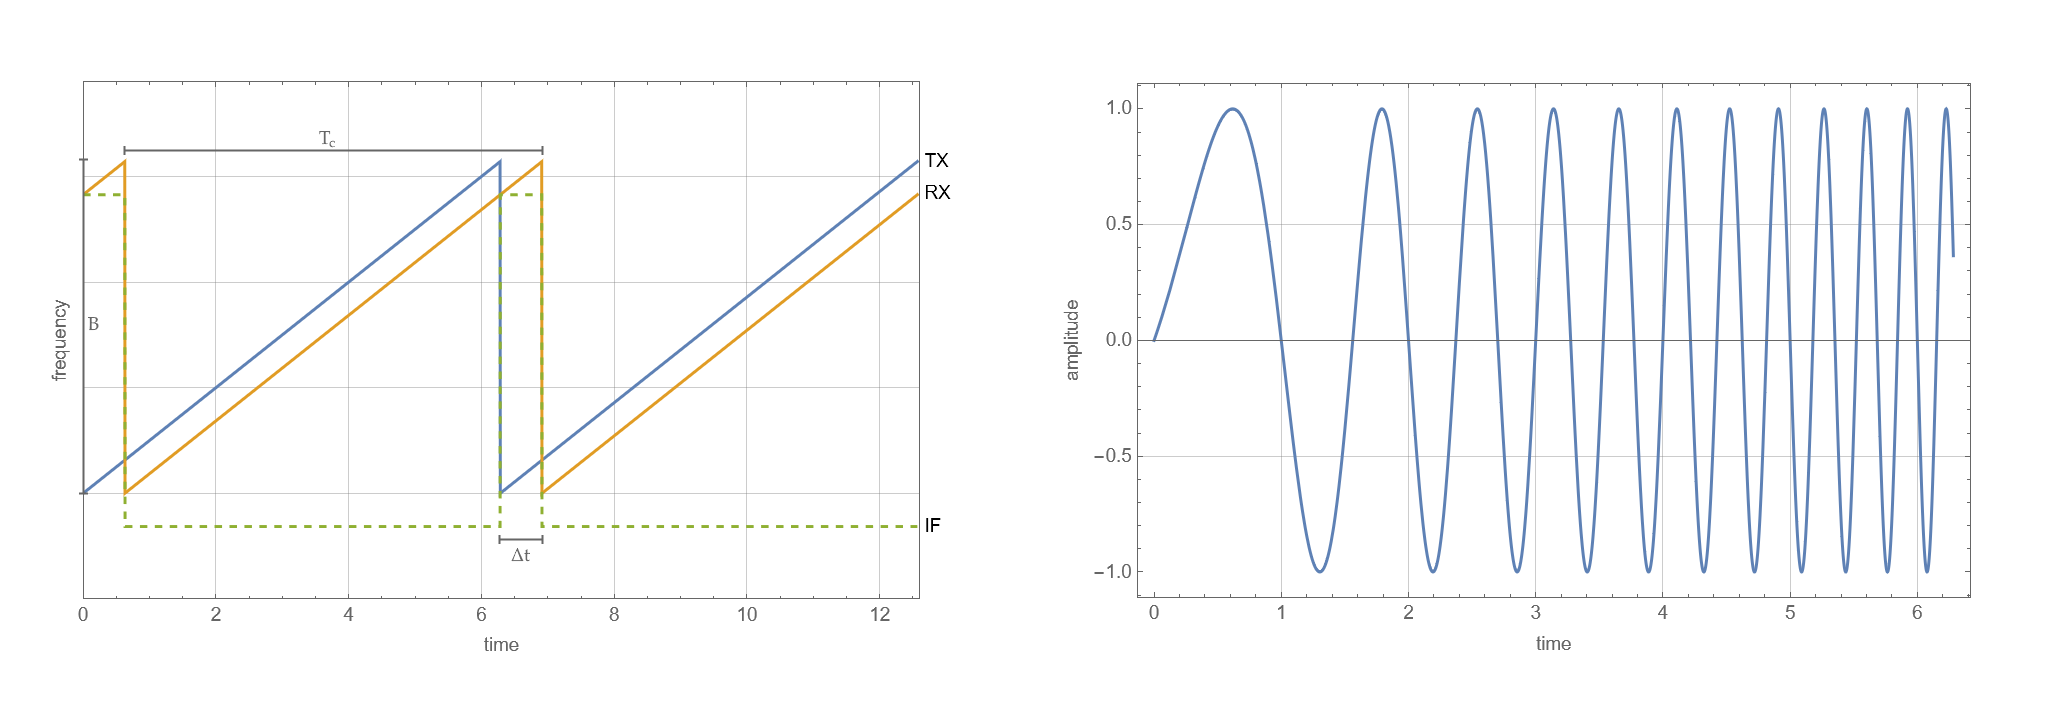
\includegraphics[width=\textwidth]{chirp-2}
	\caption{Left: transmitted (TX) and received (RX) sawtooth chirps and their difference frequency (IF). Right: illustration of TX chirp waveform (own work).}
	\label{fig:Chirp}
\end{figure}

Frequency-modulated continuous wave (FMCW) radar systems emit consecutive 'chirps' - signals whose frequency is a function of time, often a triangle or sawtooth wave. The reflected chirp arrives at a time \(\Delta t\) after emission, leading to a phase difference as shown in Fig. \ref{fig:Chirp}. The transmitted and received signals are passed through a mixer to extract their difference/intermediate frequency (IF) on which some signal processing can be performed to determine the range and velocity.

\paragraph{Range measurement.} The target range relates to the time delay and hence the intermediate frequency by
\begin{equation}
	r = \frac{c \Delta t}{2} = \frac{c f_{IF} T_c}{2 B}.
\end{equation}
In practice, there are many received signals, thus one performs a discrete Fourier transform of the IF signal to obtain a range profile, known as a range-FFT. Since the range-FFT is discrete, the range resolution is limited by the bandwidth \(B\) of the chirp:
\begin{equation}
	r_{res} = \frac{c}{2B}.
\end{equation}
With typical bandwidths ranging from \SI{1}{\mega\hertz} to \SI{1}{\giga\hertz}, FMCW radar allows for a range resolution anywhere from \SI{15}{\metre} to \SI{15}{\centi\metre}.

\paragraph{Velocity measurement.} Two targets at roughly the same range appear in the same bin on the range-FFT. Fortunately, it is possible to distinguish them by considering the phase of the signal in each bin across subsequent chirps. If a target is moving at a velocity \(v\), the phase of the IF signal changes by an amount given by
\begin{equation}
	\delta = \frac{4 \pi v T_c}{\lambda},
\end{equation}
where \(T_c\) is the chirp repetition frequency. The velocity is unambigious only if \(-\pi \le \delta \le \pi\), thus leading to a maximum velocity of
\begin{equation}
	v_{max} = \frac{\lambda}{4 T_c}.
\end{equation}
If the velocity is outwith the interval \([-v_{max}, v_{max}]\), aliasing will occur.

For multiple targets, we once again perform an FFT (Doppler-FFT) on each range bin over a sequence of chirps known as a frame. This imposes a velocity resolution given by
\begin{equation}
	v_{res} = \frac{\lambda}{2 T_f},
\end{equation}
where \(T_f\) is the time per frame.

\subsection{Radar output}
\begin{table}
	\centering
	\begin{tabular}{l|l}
		Reflectivity factor (dBZ) & Types and approximate base altitudes                                                               \\
		\midrule
		less than \(-50\)         & Cumulus (\(0.3\) to \(1.5\) \si{\kilo\metre}), altocumulus (\(2\) to \(6\) \si{\kilo\metre}), thin cirrus (\(6\) to \(12\) \si{\kilo\metre}) \\
		\(-40\) to \(-20\)        & Stratus (\(0\) to \(1.2\) \si{\kilo\metre}), altostratus (\(3\) to \(6\) \si{\kilo\metre}), thick cirrus (\(6\) to \(12\) \si{\kilo\metre})  \\
		\(-20\) and above         & Precipitation                                                                                     
	\end{tabular}
	\caption{Reflectivity factors and associated cloud types,\supercite{GorkaReflectivity} including base altitudes.\supercite{CloudTypes}.}
	\label{tbl:dBZInterpretation}
\end{table}

We mentioned the importance of the radar reflectivity factor \(Z\) in cloud classification and measuring the intensity of precipitation.
[Discuss: Z]

Further information can be obtained from Doppler velocity spectra.
[Discuss: mean, width, skew, kurtosis, drop size distribution]

\supercite{RadarMeteorology}

\subsection{Radar sensitivity}
An important metric in characterising radar systems is the \textit{sensitivity}, often defined as the minimum detectable reflectivity. 
\begin{equation}
	dBZ = C + P_r + 20\log{r}
\end{equation}
[Add units and explain this equation, plus how to get sensitivity plot.]
[\(P_r = SNR * noise power = SNR * bandwidth * kT\)...]

\begin{figure}
	\centering
	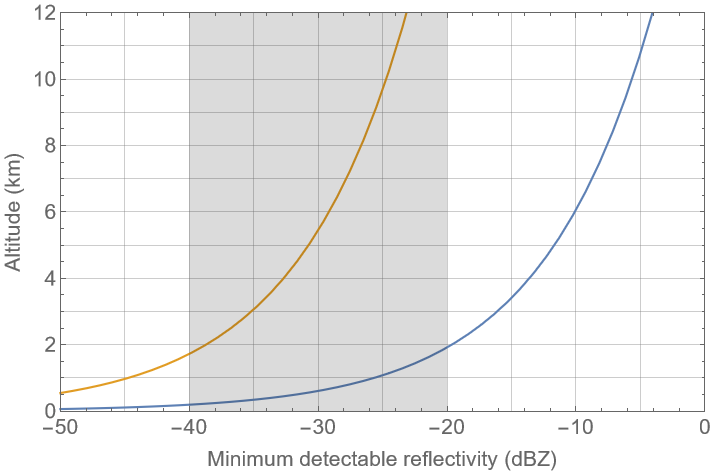
\includegraphics[width=0.5\textwidth]{sensitivity}
	\caption{Predicted minimum detectable reflectivity curve using parameters for the St. Andrews radar given in Table \ref{tbl:RadarSystems}. Assumes a signal-to-noise ratio of \(1\), a temperature of \SI{290}{\kelvin}, and \(\abs{K}^2 = 0.846\)\supercite{ComplexIndexOfRefraction} since the radar operates at \SI{94}{\giga\hertz}. \textit{To-do: temperature dependence of \(\abs{K}^2\), averaging, other radar systems, mark dBZ range of interest for clouds.} (own work)}
	\label{fig:Sensitivity}
\end{figure}

\subsection{Radar systems}
[Would like to discuss ARM here as well]

\begin{table}
	\begin{tabular}{lr|l|l|l}     & & St. Andrews\supercite{StAndrewsRadar} & BASTA\supercite{BASTA} & Huggard\supercite{HuggardRadar} \\
		\midrule
		\textbf{Frequency}        & (\si{\giga\hertz})    & \(94\)   & \(95\) & \\
		\textbf{Chirp frequency}  & (\si{\hertz})         & \(6510\) & \(\) & \\
		\textbf{Bandwidth}        & (\si{\mega\hertz})    & \(15\)   & \(\) & \\
		\textbf{Range resolution} & (\si{\metre})         & \(10\)   & \(25\) & \\

		\textbf{Transmit power}   & (\si{\deci\belm})     & \(25\)   & \(27\)--\(30\) & \\
		\textbf{Antenna gain}     & (\si{\deci\beli})     & \(52\)   & \(54\) & \\
		\textbf{Beamwidth}        & (\degree)             & \(0.43\) & \(0.4\) & \\

		\textbf{Noise figure}     & (\si{\deci\bel})      & \(5.3\)  & \(8\) &  \\
		
		\textbf{Weather constant} & (\si{\deci\belm})     & \(\)     & & \\
	\end{tabular}
	\caption{Parameters for various radar systems.}
	\label{tbl:RadarSystems}
\end{table}

\subsubsection{Solid state \SI{94}{\giga\hertz} FMCW cloud profiling radar}
The Millimetre Wave and EPR Group at the University of St Andrews has been developing a ground-based, zenith-pointing radar that operates at \SI{94}{\giga\hertz}.\supercite{StAndrewsRadar} The radar utilises solid-state electronics and two Fresnel zone plate antennas, significantly reducing the cost.

Since FMCW radar requires thousands of FFTs to be performed, the radar software is written in C and leverages both the CPU and GPU for maximum performance. Since each FFT can be performed independently, multithreading can be used to further improve throughput, through this comes at the cost of increased software complexity.\supercite{Cassidy}
Other approaches considered include specialised hardware dedicated to signal processing such as a digital signal processor (DSP) or field-programmable gate array (FPGA), though these are considerably less flexible than a conventional CPU-based design.

\subsubsection{Bistatic Radar System for Atmospheric Studies (BASTA) \SI{95}{\giga\hertz} FMCW cloud radar}
[BASTA uses FPGAs. Bandwidth and some other parameters are variable, like with the St. Andrews radar. Table \ref{tbl:RadarSystems} is a bit misleading.]

\section{Project work}
The St. Andrews radar software needs to be updated to allow for averaging, extraction of Doppler moments, and real-time output. Also, calibration and some outdoor testing needs to be performed, in particular assessing the effect of ambient temperature on radar performance. 
\paragraph{Signal averaging.} Averaging of range profiles reduces noise and increases sensitivity to low reflectivity clouds such as thin cirrus. Figure \ref{fig:Sensitivity} shows that without averaging the radar will be unable to detect any clouds above \SI{2}{\kilo\metre}.
\paragraph{Doppler moments.} Extraction of Doppler moments (mean, skew, kurtosis) provides meteorologists with more information and allows them to better study the onset of cloud formation, for example.
\paragraph{Real-time output.} Real-time saving in netCDF,\supercite{NetCDFFormat} a format widely used by meteorologists. This would allow for offline data processing.
\paragraph{Effect of ambient temperature.} Changes in ambient temperature could affect the radar performance. Solid-state devices are particularly vulnerable to thermal drift. Thermal sensors in the radar enclosure will record the ambient temperature over a long period of time (?a day, a week, two weeks?) which can be correlated to radar performance (explain).
\paragraph{Cross-check results with disdrometer.} Time permitting, a disdrometer located next to the radar could be used to collect reflectivity data which can then be compared to theoretical predictions and the output from the radar, providing a way to cross-check results.

\section{Conclusions}
[What was covered in this article?]
[Future of FMCW cloud radar, problems]

[Perhaps this article is a bit heavy on theory... need to better reference in theory section, particularly the range/velocity paragraphs.]
[Some paragraphs don't flow together very well, such as introduction -> meteorological radar.]
[Introduction is also quite light on references, doesn't really mention the scope of the article.]

\nocite{*}
\printbibliography
\end{document}
